\section{Inverse Trigonometric Functions}
If \textit{$x = \sin\theta$} then we define the inverse trigonometric function as \textit{$\sin^{-1}(x) = \theta$}, the same holds true for all other trigonometric functions.

\subsection{Properties of Inverse Trigonometric Functions}

\begin{align*}
\hspace{20mm} \sin^{-1}(\sin\theta) &= \theta  \hspace{20mm} \mathrm{cosec}^{-1}(\mathrm{cosec}\theta) = \theta\\
\hspace{20mm} \cos^{-1}(\cos\theta) &= \theta  \hspace{20mm} \mathrm{sec}^{-1}(\mathrm{sec}\theta) = \theta\\ 
\hspace{20mm} \tan^{-1}(\tan\theta) &= \theta \hspace{20mm} \cot^{-1}(\cot\theta) = \theta \\ \\
\hspace{20mm} \sin(\sin^{-1}(x)) &= x  \hspace{20mm} \mathrm{cosec}(\mathrm{cosec}^{-1}(x)) = x\\
\hspace{20mm} \cos(\cos^{-1}(x)) &= x  \hspace{20mm} \mathrm{sec}(\mathrm{sec}^{-1}(x)) = x\\ 
\hspace{20mm} \tan(\tan^{-1}(x)) &= x \hspace{20mm} \cot(\cot^{-1}(x)) = x 
\end{align*}

\begin{figure}[ht]
    \centering
    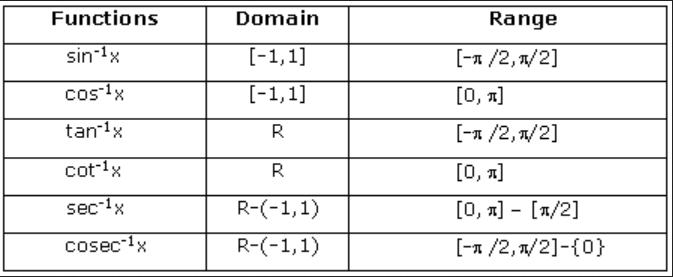
\includegraphics{inverse_trigonometry}
    \caption{Domain and range of inverse trigonometric functions}
    \label{inverse_trig}
\end{figure}

\begin{align*}
\hspace{20mm} \sin^{-1}(x) \hspace{5mm} &= \hspace{5mm} \cos^{-1}\sqrt{1-x^2} \hspace{5mm} = \hspace{5mm}  \tan^{-1}\frac{x}{\sqrt{1-x^2}}\\
\hspace{20mm} \cos^{-1}(x) \hspace{5mm} &= \hspace{5mm} \sin^{-1}\sqrt{1-x^2} \hspace{5mm} = \hspace{5mm}  \tan^{-1}\frac{\sqrt{1-x^2}}{x}\\
\hspace{20mm} \tan^{-1}(x) \hspace{5mm} &= \hspace{5mm} \sin^{-1}\frac{x}{\sqrt{1+x^2}} \hspace{5mm} = \hspace{5mm}  \cos^{-1}\frac{1}{\sqrt{1+x^2}}
\end{align*}

\begin{align*}
\hspace{20mm} \sin^{-1}(-x)  \hspace{5mm} &= \hspace{5mm} -\sin^{-1}(x) \hspace{5mm} x \in [-1,1] \\
\hspace{20mm} \cos^{-1}(-x)  \hspace{5mm} &= \hspace{5mm} \pi - \cos^{-1}(x) \hspace{5mm} x \in [-1,1] \\
\hspace{20mm} \tan^{-1}(-x)  \hspace{5mm} &= \hspace{5mm} -\tan^{-1}(x) \hspace{5mm} x \in \mathrm{R} \\
\hspace{20mm} \mathrm{cosec}^{-1}(-x)  \hspace{5mm} &= \hspace{5mm} -\mathrm{cosec}^{-1}(x) \hspace{5mm} x \in (-\infty,-1] \cup [1,\infty)\\
\hspace{20mm} \mathrm{sec}^{-1}(-x)  \hspace{5mm} &= \hspace{5mm} \pi-\mathrm{sec}^{-1}(x) \hspace{5mm} x \in (-\infty,-1] \cup [1,\infty)\\
\hspace{20mm} \cot^{-1}(-x)  \hspace{5mm} &= \hspace{5mm} \pi -\cot^{-1}(x) \hspace{5mm} x \in \mathrm{R} \\ \\
\hspace{20mm} \sin^{-1}(\frac{1}{x})  \hspace{5mm} &= \hspace{5mm} \mathrm{cosec}^{-1}(x) \hspace{5mm} x \in (-\infty,-1] \cup [1,\infty)\\
\hspace{20mm} \cos^{-1}(\frac{1}{x})  \hspace{5mm} &= \hspace{5mm} \mathrm{sec}^{-1}(x) \hspace{5mm} x \in (-\infty,-1] \cup [1,\infty)\\
\tan^{-1}(1/x) \hspace{5mm} &= \hspace{5mm}
\begin{cases}
\cot^{-1}(x), \hspace{5mm}   x > 0 \\
\cot^{-1}(x) - \pi, \hspace{5mm} x < 0\\
\end{cases}
\end{align*} 


\begin{align*}
\hspace{20mm} \sin^{-1}(x) \hspace{5mm} &+ \hspace{5mm} \cos^{-1}(x) \hspace{5mm} = \hspace{5mm} (\pi/2)\\
\hspace{20mm} \tan^{-1}(x) \hspace{5mm} &+ \hspace{5mm} \cot^{-1}(x) \hspace{5mm}  = \hspace{5mm} (\pi/2)\\
\hspace{20mm} \sec^{-1}(x) \hspace{5mm} &+ \hspace{5mm} \mathrm{cosec}^{-1}(x) \hspace{5mm} = \hspace{5mm} (\pi/2) \\ \\
\hspace{20mm} \tan^{-1}(x) \hspace{5mm} &+ \hspace{5mm} \tan^{-1}(y) \hspace{5mm} = \hspace{5mm} \tan^{-1}\frac{x+y}{1-xy}\\
\hspace{20mm} \tan^{-1}(x) \hspace{5mm} &- \hspace{5mm} \tan^{-1}(y) \hspace{5mm} = \hspace{5mm} \tan^{-1}\frac{x-y}{1+xy}\\
\hspace{20mm} 2\tan^{-1}(x) \hspace{5mm} &= \hspace{5mm} 
\begin{cases}
2\sin^{-1}\frac{2x}{1+x^2}, \hspace{5mm}   x > 0 \\
\cos^{-1}\frac{1-x^2}{1+x^2}, \hspace{5mm} x < 0\\
\end{cases}
\end{align*}

\pagebreak
\subsection{Expressions and suggested substitutions}
\hspace{40mm} \textbf{Expression} \hspace{20mm} \textbf{Substitution} \hspace{10mm}

\begin{align*}
\hspace{20mm} a^2 &+ x^2 \hspace{20mm} x=a\tan\theta \hspace{5mm} or \hspace{5mm} x=a\cot\theta\\
\hspace{20mm}  a^2 &- x^2  \hspace{20mm} x=a\sin\theta \hspace{5mm} or \hspace{5mm} x=a\cos\theta\\
\hspace{20mm}  x^2 &- a^2  \hspace{20mm} x=a \mathrm{cosec}\theta \hspace{3mm} or \hspace{5mm} x=a\sec\theta \\
\hspace{25mm}  \sqrt{\frac{a-x}{a+x}} \hspace{3mm}  &or \hspace{3mm}\sqrt{\frac{a+x}{a-x}}  \hspace{8mm} x=a\cos2\theta \hspace{5mm}\\
\hspace{25mm}  \sqrt{\frac{a^2-x^2}{a^2+x^2}} \hspace{3mm} &or \hspace{3mm}\sqrt{\frac{a^2+x^2}{a^2-x^2}}  \hspace{6mm} x=a^2\cos2\theta \hspace{5mm}
\end{align*}
